\documentclass{article}
\usepackage{graphicx} % Required for inserting images
\usepackage{float}
\usepackage{url}

\title{CTA200 Assignment \#3}
\author{Damon}

\begin{document}

\section*{Question \#1}


\begin{figure}[H]
  \centering
  \begin{minipage}[b]{0.45\textwidth}
    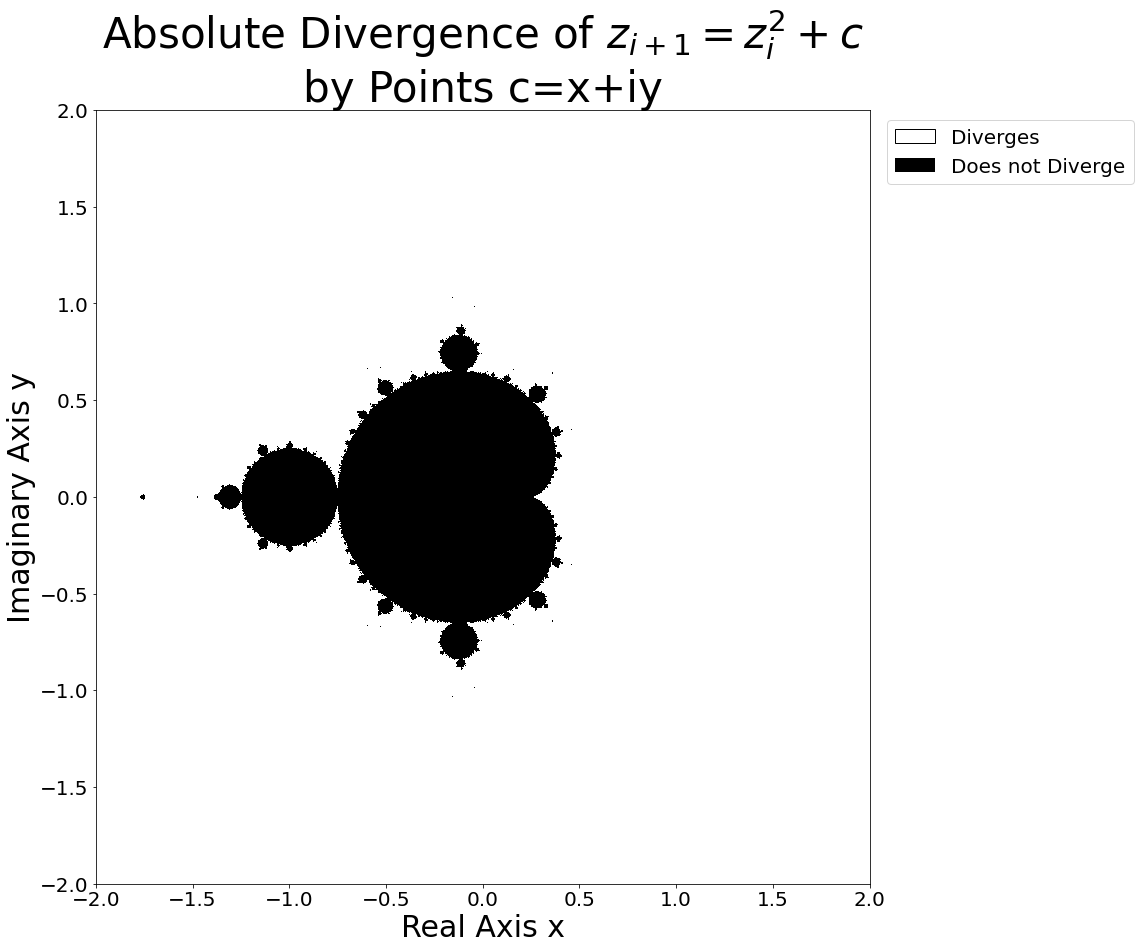
\includegraphics[width=\textwidth]{bw.png}
    %\caption{Absolute}
  \end{minipage}
  \hfill
  \begin{minipage}[b]{0.5\textwidth}
    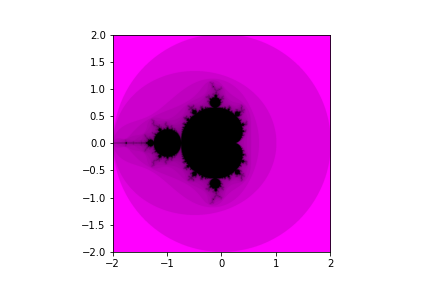
\includegraphics[width=\textwidth]{colour.png}
    %\caption{Gradient}
  \end{minipage}
\end{figure}

The above graphs are the results from question 1. They were made by plotting points in a grid in the range -2 to 2 on the real axis (x) and -2i to 2i on the imaginary axis (y) based on their divergence to the equation:
\[z_{i+1} = z_i^2 + c\]
where $c = x+iy$ and $z_0 = 0$.
\\This was done with a resolution of 1025x1025 pixels, and a maximum number of iterations of 255. When a value $z_i$ exceeded a magnitude of 2 ($|z_i| > 2$), this is counted as divergence. If iterating this process on a point does not cause it to diverge over the number of iterations, it is counted as not diverging.
\\All code is written in Python, with the main code for iteration and returning the number of iterations to diverge in \texttt{iteration.py}, which is imported and used in the main Jupyter notebook file \texttt{question\_1.ipynb}.
\\The left image shows absolute divergence of points, meaning strictly whether a point diverged over the maximum number of iterations or not. In this image, a point diverging is coloured white, while a point not diverging is coloured black.
\\The right image has a gradient for the number of iterations to diverge, with the maximum (255) being no divergence over the iterations. This gradient is based on a logarithmic scale, visible on the very right of the image, with high numbers of iterations or no divergence being more black and more quickly diverging points being more pink (towards RGB (255, 0, 255)).
\\In both images you can see a complicated fractal pattern, with more intricate details visible in the gradient image.

\section*{Question \#2}

\begin{figure}[H]
    \centering
    \begin{minipage}[b]{0.48\textwidth}
        \centering
        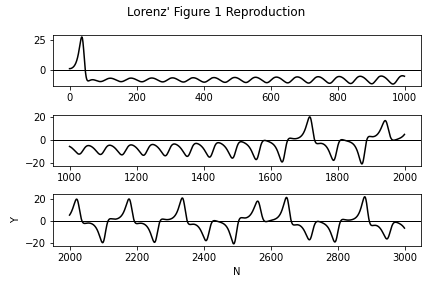
\includegraphics[width=\textwidth, height=4cm, keepaspectratio]{q2_fig1.png}
        \\[2ex]
        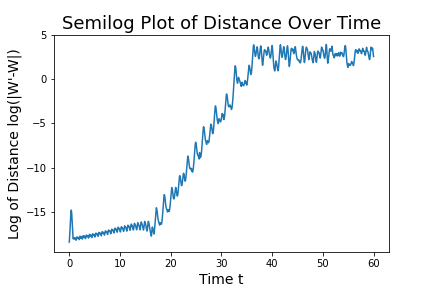
\includegraphics[width=\textwidth, height=4cm, keepaspectratio]{q2_fig3.png}
    \end{minipage}
    \hfill
    \begin{minipage}[b]{0.48\textwidth}
        \centering
        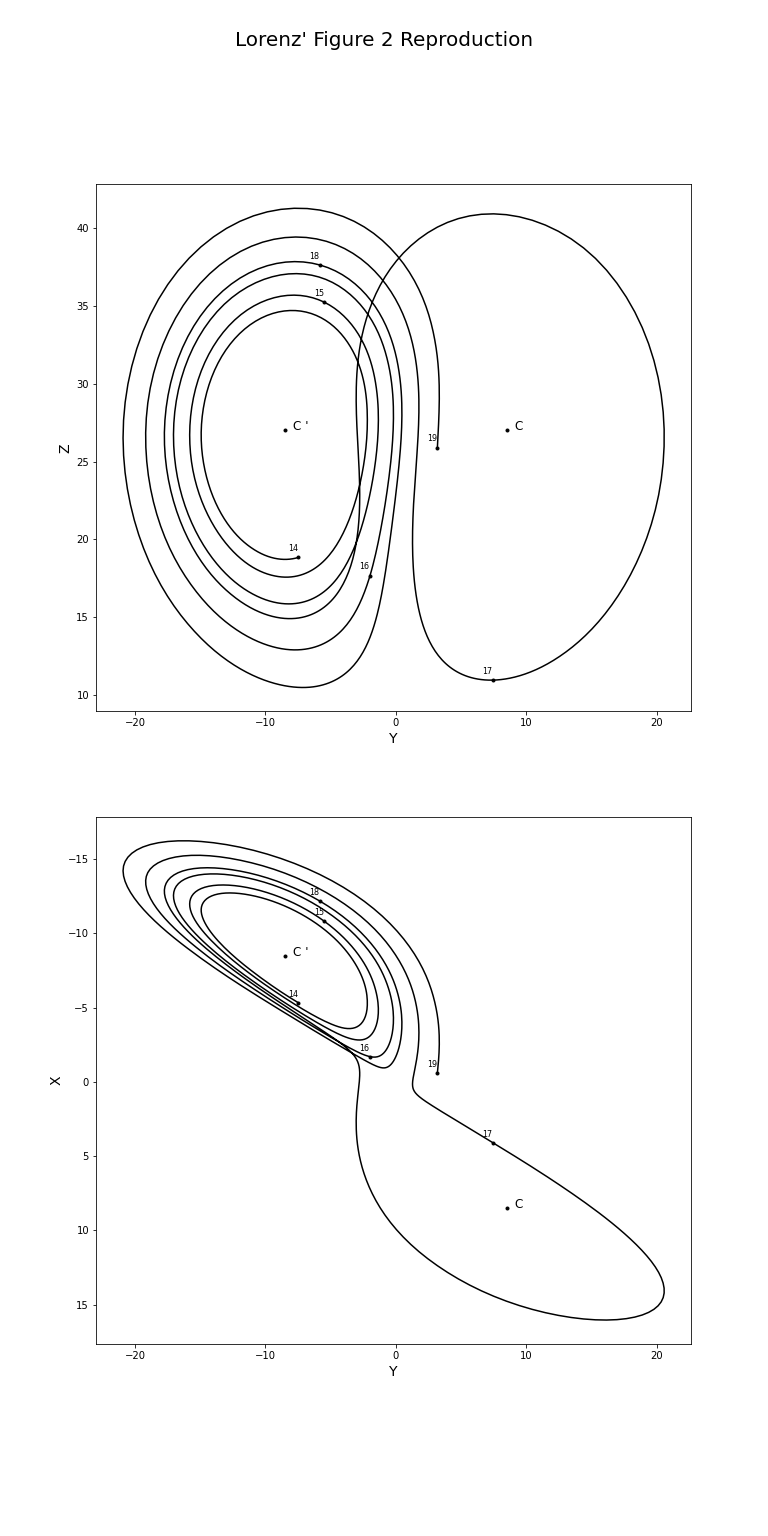
\includegraphics[width=\textwidth, height=10cm, keepaspectratio]{q2_fig2.png}
    \end{minipage}
\end{figure}

These above images are the results from question 2. They are results from analysis of the given equations (originally by Edward Lorenz in his paper "Deterministic Nonperiodic Flow" - \url{https://journals.ametsoc.org/view/journals/atsc/20/2/1520-0469_1963_020_0130_dnf_2_0_co_2.xml}):
\[\dot{X} = -\sigma (X - Y)\]
\[\dot{Y} = rX - Y - XZ\]
\[\dot{Z} = -bZ + XY\]
with $\sigma=10$, $r=28$, $b = \frac{8}{3}$, and $W = (X, Y, Z)$.
\\This system was solved using the \texttt{solve\_ivp} function from SciPy, over the time interval $t=0$ to $t=60$ with initial conditions $W_0 = (0, 1, 0)$ as well as $W_0' = W_0+(0, 1e-8, 0) = (0, 1.00000001, 0)$.
\\The top left plot shows the results of this solution (with initial conditions $W_0$) for $Y$ from $t=0$ to $t=30$ (written instead with $N = t/\Delta t$ ($\Delta t = 0.01$)). This is a recreation of Lorenz' figure 1 plot in the given paper. It is mostly the same as Lorenz' plot, but deviates slightly towards the end.
\\The right plots show the results (with initial conditions $W_0$) in Y-Z and Y-X phase space, from $t=14$ to $t=19$ (with each integer time value in this range labeled). It also shows the points of states of steady convection $C$ and $C'$ as given in the paper. This is a recreation of Lorenz' figure 2 plot, and is similarly mostly consistent, but deviates somewhat from Lorenz' plots. In both of these, there is one more concentric loops on the left side and one less on the right in mine versus Lorenz' plots. These difference as well as the difference in figure 1 could be due to being able to use higher precision on modern computers, while this paper is from over 60 years ago. In this way, small errors from lack of precision would compound, leading to the visually noticeable differences in plots here. 
\\The bottom left plot shows a semilog plot of the differences between the results from initial conditions of $W_0$ and $W_0'$ over time. The x axis is time and the y axis is the a logarithmic scale of the absolute value of the distance between the results $W'$ and $W$. From this, you can see the beginning and end as mostly flat, with a linear increase in the middle, indicating exponential growth in this distance. This is consistent with the results found by Lorenz.

\end{document}
